\chapter{PHÂN TÍCH}
\section{Mô Hình}

\subsection{Mô hình triển khai hệ thống}
	\begin{center}
	\begin{figure}[H]
		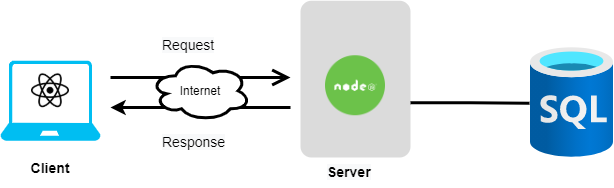
\includegraphics[width=17cm]{{./imgs/implement_tech_diagram}}
		\caption{Mô hình triển khai}
	\end{figure}
	\end{center}
	
\subsection{Mô tả sơ đồ}
\begin{center}
\begin{longtabu} to \textwidth {| m{5cm} | m{5cm} | m{5cm} |}
\caption{Mô tả sơ đồ} \\
\hline \textbf{Tên} & \textbf{Mô tả} & \textbf{Công nghệ} \\ \hline
\endfirsthead
\hline \textbf{Tên} & \textbf{Mô tả} & \textbf{Công nghệ} \\ \hline
\endhead
\hline
\endfoot
Client & Là nơi User tương tác gửi các yêu cầu, các chức năng và dữ liệu đến máy chủ để máy chủ xử lý yêu cầu và trả về kết quả & ReactJS
\\ \hline
Server & Là chấp nhận tất cả yêu cầu hợp lệ từ Client, sau đó trả về kết quả đã tính toán & NodeJS
\\ \hline
Database & Là nơi lưu trữ dữ liệu & MySQL
\\ \hline
Request, Response & Gửi và nhận dữ liệu thông qua Internet & Giao thức: TCP/IP, HTTP Protocol
\\ \hline
\end{longtabu}
\end{center}

\section{Sơ Đồ Use Case}
\subsection{Tổng quan}
	\begin{center}
		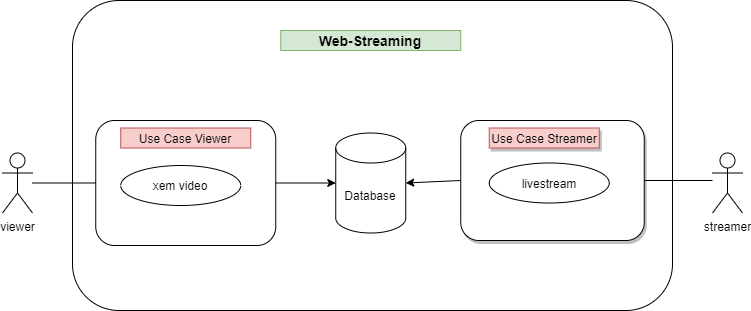
\includegraphics[width=17cm]{{./imgs/usecase_model.png}}
	\end{center}

\subsection{Use case cho viewer}
	\begin{center}
		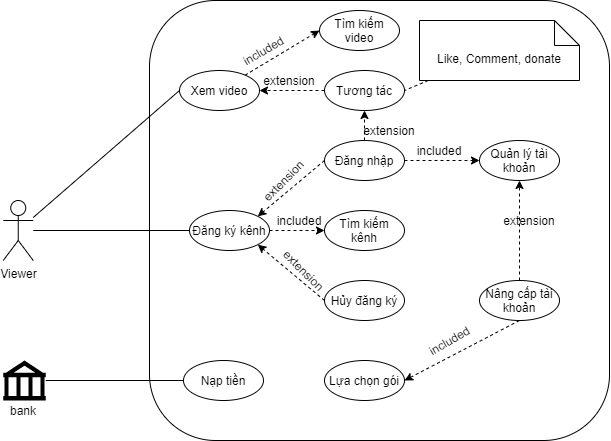
\includegraphics[width=17cm]{{./imgs/usecase_viewer.png}}
	\end{center}
	
\subsection{Use case cho streamer}
	\begin{center}
		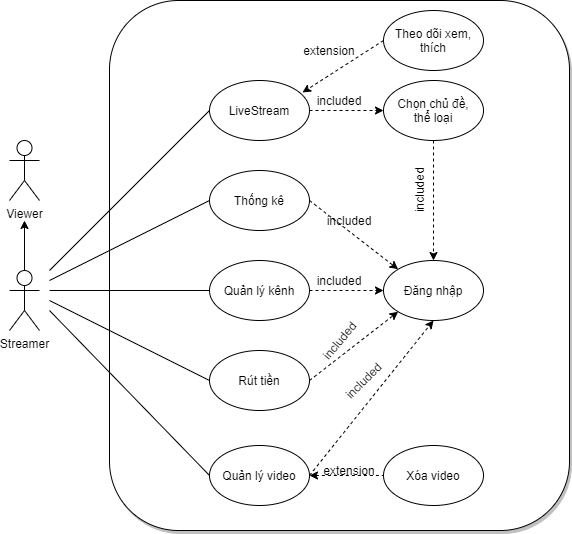
\includegraphics[width=17cm]{{./imgs/usecase_streamer.png}}
	\end{center}
		
	
\section{Đặc Tả Hệ Thống}
\subsection{Chi tiết dành cho Viewer}

 \begin{center}
\begin{longtabu} to \textwidth {| m{5cm} | m{5cm} | m{5cm} |}
\caption{Mô tả chi tiết Use Case Viewer}  \\ 
\hline \textbf{Tên chức năng} & \textbf{Mô tả} & \textbf{Ghi chú} \\ \hline
\endfirsthead
\hline \textbf{Tên chức năng} & \textbf{Mô tả} & \textbf{Ghi chú} \\ \hline
\endhead
\hline
\endfoot
Đăng ký & Người dùng đăng ký tài khoản để truy cập vào hệ thống  &
\\ \hline
Đăng nhập/Đăng xuất &  Bước đầu tiến khi vào một ứng dụng và thoát ứng dụng & 
\\ \hline
Menu & Danh sách các video, kênh và tài khoản được đưa ra tuy theo sở thích, lượt xem cho người dùng & Có thể tự động \quotes{play} theo kênh đề xuất
\\ \hline
Quản lý tài khoản & Thêm, cập nhật thông tin cá nhân của tài khoản & 
\\ \hline
Nâng cấp tài khoản & Mua các gói trả phí & 
\\ \hline
Chuyển đổi tiền tệ & Giúp người dùng nạp và rút tiền từ tài khoản vào thẻ ngân hàng & Có thể liên kết gián tiếp qua các ứng dụng thanh toán trực tuyến (ZaloPay, Momo,\dots)
\\ \hline
Kênh đăng ký & Danh sách những kênh yêu thích & Nhận được thông báo khi kênh đăng hoạt động 
\end{longtabu} 
\end{center}
   
\subsection{Chi tiết dành cho Streamer}
\begin{center}
\begin{longtabu} to \textwidth {| m{5cm} | m{5cm} | m{5cm} |}
\caption{Mô tả chi tiết Use Case Streamer} \\
\hline \textbf{Tên chức năng} & \textbf{Mô tả} & \textbf{Ghi chú} \\ \hline
\endfirsthead
\hline \textbf{Tên chức năng} & \textbf{Mô tả} & \textbf{Ghi chú} \\ \hline
\endhead
\hline
\endfoot
Đăng nhập/Đăng xuất &  Bước đầu tiến khi vào một ứng dụng và thoát ứng dụng  &
\\ \hline
Live Stream &  Nơi mà streamer dùng để tạo các video và chia sẻ trưc tuyến tới người xem & Mỗi tài khoản được cấp cho một mã phòng nhất định
\\ \hline
Quản lý kênh & Nơi lưu trữ dữ liệu chính của hệ thống & Có thể sử dụng nhiều hệ cơ sở dữ liệu khác nhau (SQL Server, MySQL, MongoDB..)
Mỗi service có một hệ cơ sở dữ liệu riêng biệt
\end{longtabu}
\end{center}


